\chapter{虚拟实验室与评价协议}
\label{ch:sim}

本章要判定的量是：一次数值比较能不能称为这台蒸烤一体机的感知成立。判据是真值与估计器是否隔离、指标是否在真值上计算、以及没有跑过的套件是否被排除在句子之外。

主对照的因子格子不变：三种食品、三种厚度、两个初温、三个含水、三种非均质、四个策略。每个格子 30 个种子的 19440 行已经落盘。S0 在 30 mm、对偶、初温 \(5^\circ\mathrm{C}\)、含水 0.72、均匀场上，把每个原型的 6 个种子用 16 个控制体和 8 个控制体各积一次。S2 只在 30 mm、肉糜、同一初温和含水上做边界扫描，每个因子 40 个种子，合计 480 行。S3、T2、T3 仍未运行。同一格子按 30000 个种子放大的脚本没有跑完，未完成的格子不引用。

\section{双模型原则}

\paragraph{要判定的量}
真值模型 T 与在线模型 E 是否共用同一套参数。共用则结果只说明离散格式自洽。

\paragraph{继承的文献层与不继承的层}
隔离继承估计理论里“观测以外的状态不可读” \cite{ozisik2000,evensen2003}。不继承把同一程序里的内部数组叫做不可见：不可见必须落在接口上。

规格中的 T 是一维或二维多孔介质方程，网格细于在线模型，参数从先验抽样并含空间非均质。E 是两节点或神经算子，初始化为类别先验，不得读取 T 的参数真值。同构试验只做数值自检，不进入主表。

本次没有这个配对。积分器就是十六条控制体，估计器是附在同一循环里的标量跟踪器。热阻更新还读取由真值温差构成的参照。因此本章的数字是“一个工程核上四条策略的差别”，不是“T 与 E 异构时的感知误差”。D21 所要求的同构—异构对照没有日志，也不会出现在结论句里。

腔体流动不在每个控制周期里重算。规格把少量外部流动收成 \(h(|v|)\)、角系数和混合时间的边界库。本次 \(h=12+55u_{\mathrm{fan}}\) 是线性式，不是边界库。

\paragraph{本节不能推出的结论}
核内部自洽，不能写成冷点估计已经在异构真值上通过。

\section{四套仿真，不混在一个总数里}

\paragraph{要判定的量}
一条轨迹属于哪一套，能不能进入主结论的分母。

\begin{table}[ht]
\centering
\caption{套件与本次是否运行}
\begin{tabularx}{\textwidth}{lXr}
\toprule
套件 & 规格中要回答的问题 & 本次 \\
\midrule
S0 格式 & 网格减半后决策状态的变化 & 18 条配对已运行 \\
S1 主对照 & 四条策略的进度误差 & 已运行 \\
S2 边界与失效 & 探针、遮挡、缺通道、脂肪层、一次开门 & 480 行已运行 \\
S3 教师 & 训练算子并做干预位移 & 未运行 \\
\bottomrule
\end{tabularx}
\end{table}

S1 的因子是 3 个原型、3 个厚度、2 个初温、3 个含水、3 个非均质档、30 个种子。乘积
\begin{equation}
3\times 3\times 2\times 3\times 3\times 30=4860.
\end{equation}
四个策略各 4860 行，合计 19440 行。较早写过的 1620 少乘了非均质的 3 档。日志与 4860 一致。这 19440 行是同一数值过程的样本，不是独立烹饪，也不是 S3 的扩充。每行 \texttt{augmented=false}，\texttt{source=simulation}。

S2 落在 30 mm、肉糜、初温 \(5^\circ\mathrm{C}\)、含水 0.72。探针只对照对偶与无探针。表面读数在开局后的 0、15、30、60 s 内保持初值，用来代替热像遮挡；核没有热像通道。质量通道只改腔温比例的蒸汽阈值，对偶这条不读它。脂肪层沿用主对照的导热缺损。开门是 300 s 时表面控制体下降 \(15^\circ\mathrm{C}\)。每档 40 个种子。探针五档、噪声倍数和管温贴近屏障没有单独的水平，因为窗是固定的，噪声倍数不改变对偶的更新规则，加热器平衡点又低于削减阈值。S3 的高保真约 360 条和扩充 \(10^4\) 条没有生成。

\paragraph{本节不能推出的结论}
不能把 19440 写成实验次数。S2 的 480 行回答的是这一条 30 mm 设定上的边界，不能并进 S1 的分母。S3 仍然不进入任何分母。

\section{主因素}

\begin{table}[ht]
\centering
\caption{S1 因子的实际取值}
\begin{tabularx}{\textwidth}{llX}
\toprule
因素 & 水平 & 在核里的实现 \\
\midrule
原型 & 肉糜、土豆、面团 & 只改活度尺度 \\
厚度 & 15 mm、30 mm、50 mm & 网格间距与时间常数 \\
初温 & 5\(^\circ\mathrm{C}\)、20\(^\circ\mathrm{C}\) & 均匀初值；种子 7 的演示轨迹另取 8\(^\circ\mathrm{C}\)，不在这 4860 行里 \\
含水 & 0.64、0.72、0.80 & 均匀初值 \\
非均质 & 0、1、2 & 0 均匀；1 为沿厚度 \(\pm 4^\circ\mathrm{C}\)；2 为下标 5 的导热乘 0.45 \\
种子 & 0--29 & 噪声散列的整数部分为 \(1000+\mathrm{seed}+17\times\) 原型编号 \\
\bottomrule
\end{tabularx}
\end{table}

四条策略：

\begin{enumerate}
\item 开环。按厚度给菜单时间，中途不改。对应规格中的 B0。
\item 腔温比例。只跟踪带噪腔温，不停机。它不是带湿度阈值的完整腔体闭环，只保留了 B1 的“不看冷点”这一条。
\item 无探针。饱和线性加热律，没有蒸汽窗。它不是 CasADi 求解的预测控制，只保留了 B2 的“不主动探针”。
\item 对偶。同一加热律，加 \([150,190)\) 秒的窗和厚件方差否决。它不是 B3 的集合估计、探针库打分、因果解释和二次投影。
\end{enumerate}

消融规格包括去掉质量、去掉热像、去掉 P4、去掉结壳到热阻的边、去掉屏障。这些没有单独的日志列。屏障本身在本次加热器平衡点上不动作，所以“去掉屏障”也无法从这批轨迹里看出差别。

\paragraph{本节不能推出的结论}
因子表上的“脂肪”不是二维脂肪几何。非均质档 2 是一个控制体的系数。

\section{指标}

所有已经计算的指标都在这个核的场上，不是在另一个隐藏真值上。
\begin{align}
e_{\alpha}&=\alpha_m(t_{\mathrm{stop}})-0.85,\\
E&=\sum u_{\mathrm{heat}}\,\Delta t_{\mathrm{record}}.
\end{align}
\(t_{\mathrm{stop}}\) 由策略自己决定。开环停在菜单终点。腔温比例不停，摘要里的停止时刻落在时域终点 3300 s。\(e_{\alpha}<0\) 表示停在设计线之下。\(+0.150\) 是 \(\alpha_m=1\) 相对 0.85 的上沿，不是测量精度。

规格中还有场的 \(L^2\) 误差、终止时的温度标准差、安全越界次数和探针前后 \(\log\det\vect{\Sigma}\) 的差。这些列不在摘要里。不能用能量或 \(e_{\alpha}\) 代替它们。

规格中的成功准则是：对偶的提前比例低于开环和腔温比例；对偶相对无探针的场误差下降且探针确实降低协方差；越界次数在有屏障时为零、去掉屏障后为正；因果模型的干预位移优于黑箱；50 mm 允许失败，但必须输出宽区间并拒绝单点剩余时间。

对照本次日志，能说的只有第一句的一部分，而且方向与准则不完全相同。总体提前比例：开环 0.667，腔温比例 0.222，无探针 0.944，对偶 0.902。对偶低于开环，但高于腔温比例。腔温比例的低提前比例来自不停机和持续加热，中位能量 3310，中位 \(e_{\alpha}=+0.150\)。它不是更准的停止，而是把进度推到饱和。对偶相对无探针，总体中位数从 \(-0.467\) 到 \(-0.313\)，提前比例从 0.944 到 0.902。改善集中在 30 mm：无探针中位 \(-0.527\)，对偶 \(-0.080\)。15 mm 上对偶 \(-0.417\)、无探针 \(-0.367\)，探针没有优势。50 mm 上对偶 \(-0.598\)、无探针 \(-0.627\)，两者都停在设计线之下，对偶只略高，而且提前比例都是 1。50 mm 没有输出“拒绝单点剩余时间”的区间，因为界面不在这条日志里。

其余三条准则没有对象：没有场的 \(L^2\)，没有越界计数，没有干预位移。

\paragraph{本节不能推出的结论}
总体中位数不能代替按厚度分开的结论。薄件、中等厚度和厚件的排序不同。

\section{统计与图表}

统计量是中位数、十分位、九十分位和提前比例。不报告无法由种子复现的相对提升百分比。下面五张图都是这一份 S1 日志的图，不是独立实验，也不是浏览器副本。

\begin{figure}[ht]
\centering
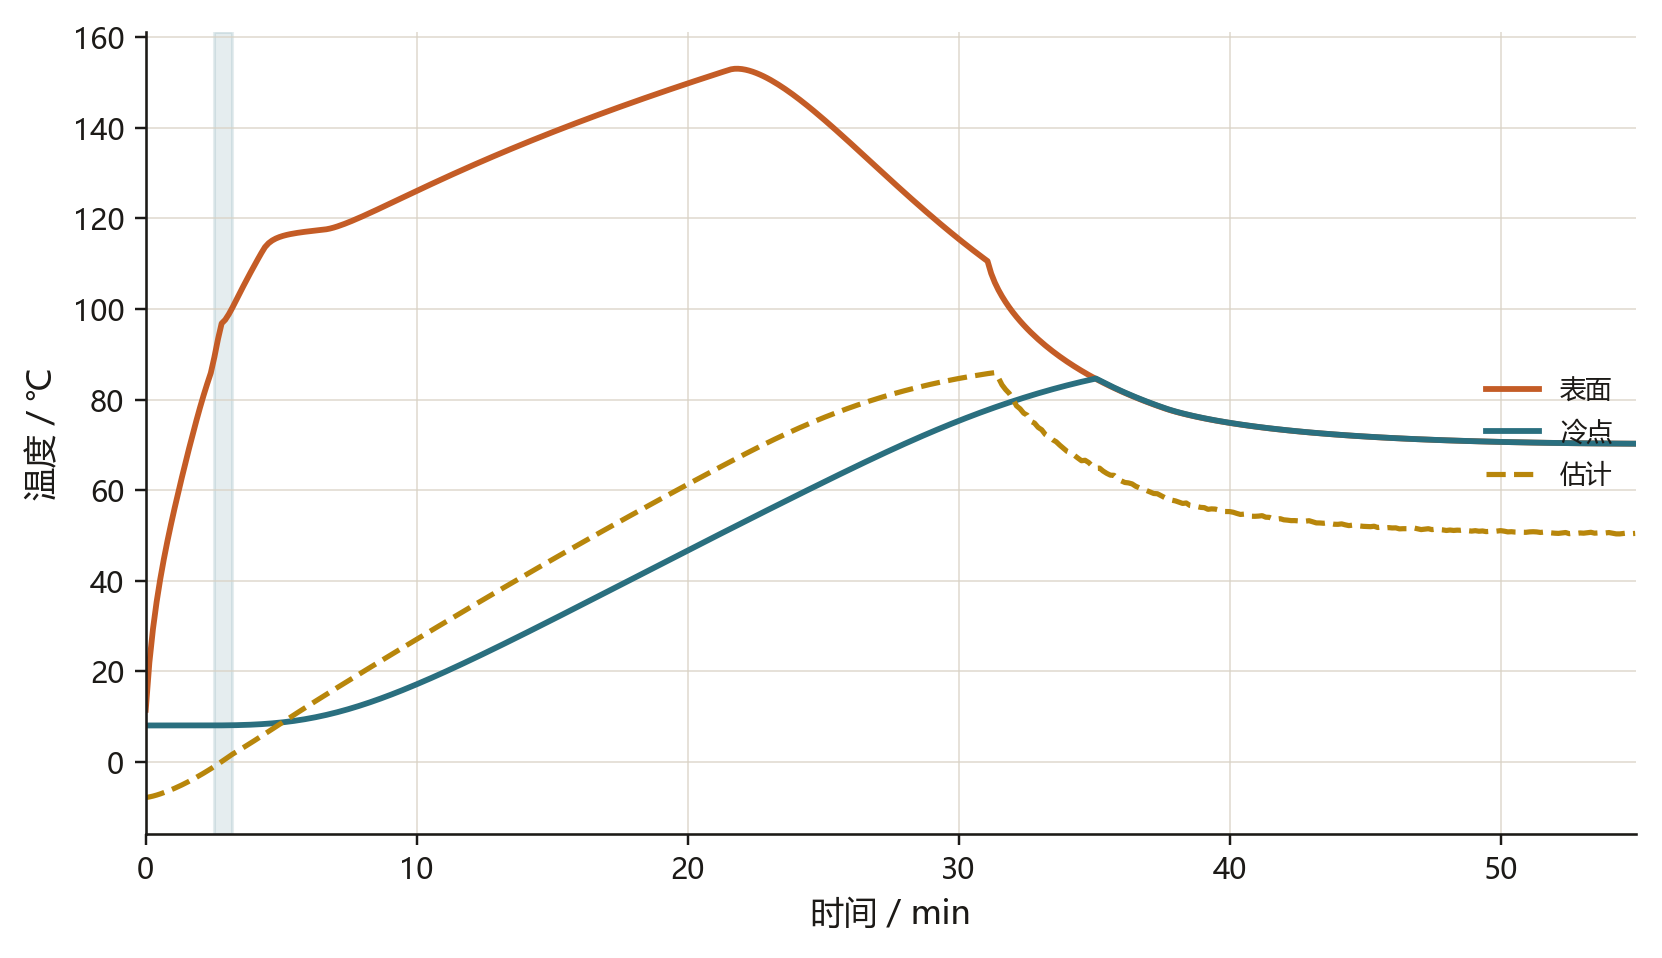
\includegraphics[width=0.86\textwidth]{D1_temperature.png}
\caption{D1。肉糜、30 mm、种子 7、对偶策略的表面温度、冷点温度和估计冷点，时间以分钟计。这是一条轨迹，不是中位数。它不能支持物理实验、二维脂肪几何或浏览器副本的温度。}
\end{figure}

\begin{figure}[ht]
\centering
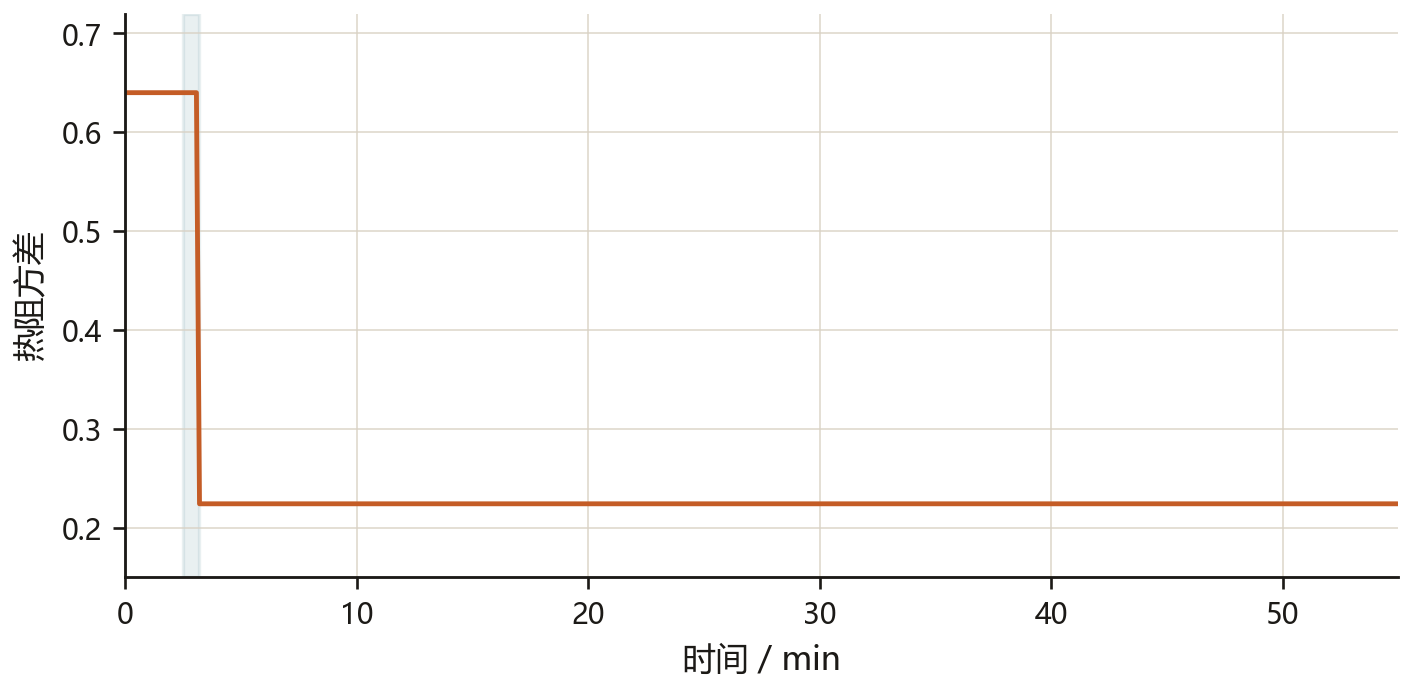
\includegraphics[width=0.86\textwidth]{D6_variance.png}
\caption{D6。同一条轨迹的热阻方差。192 s 处从 0.64 降到 0.224。降幅等于规则中的乘子 0.35，不是 Fisher 信息的特征值。不能据此比较 P0、P1、P2、P4。}
\end{figure}

\begin{figure}[ht]
\centering
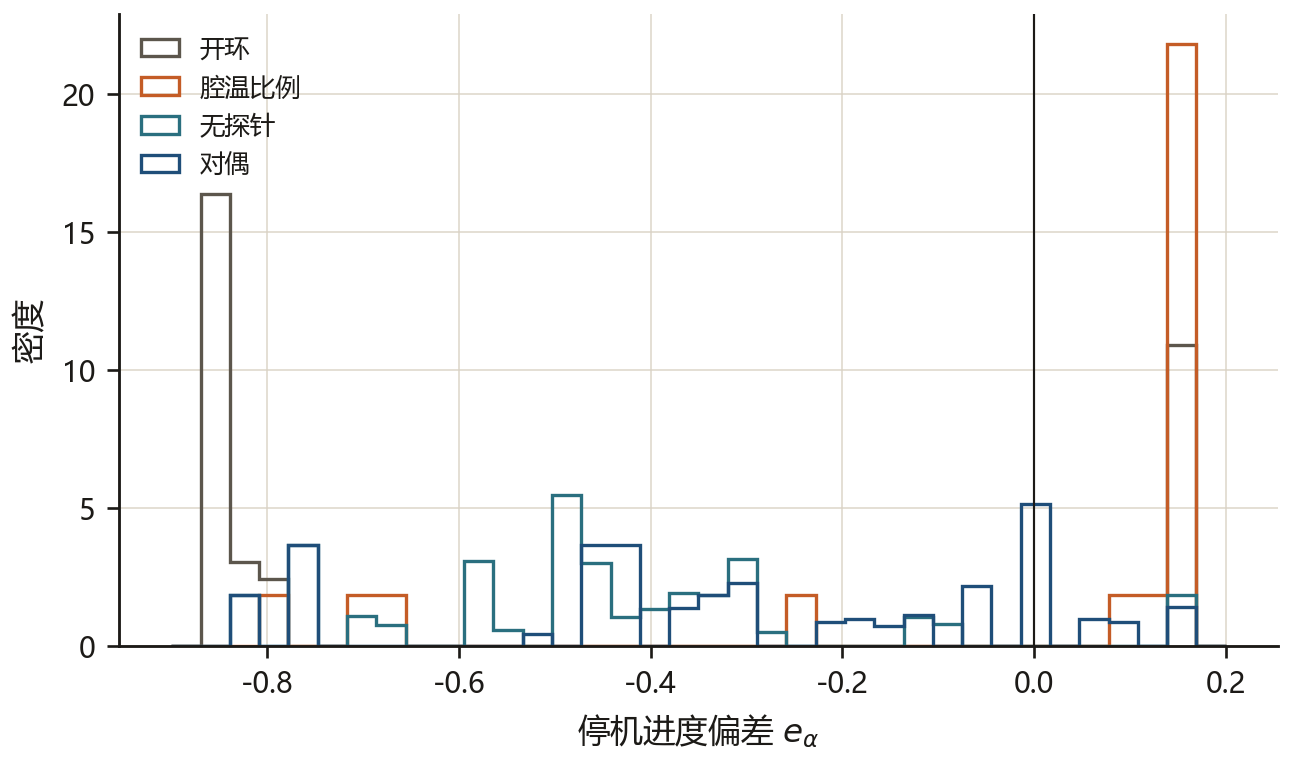
\includegraphics[width=0.86\textwidth]{D10_policy.png}
\caption{D10。四个策略的 \(e_{\alpha}\) 分布，每个策略 4860 条。零线是设计线。腔温比例的质量堆在 \(+0.15\)。这张图不能单独说明能耗，能耗在交叉表里，而且不能在没有 D10 的情况下单独作为结论。}
\end{figure}

\begin{figure}[ht]
\centering
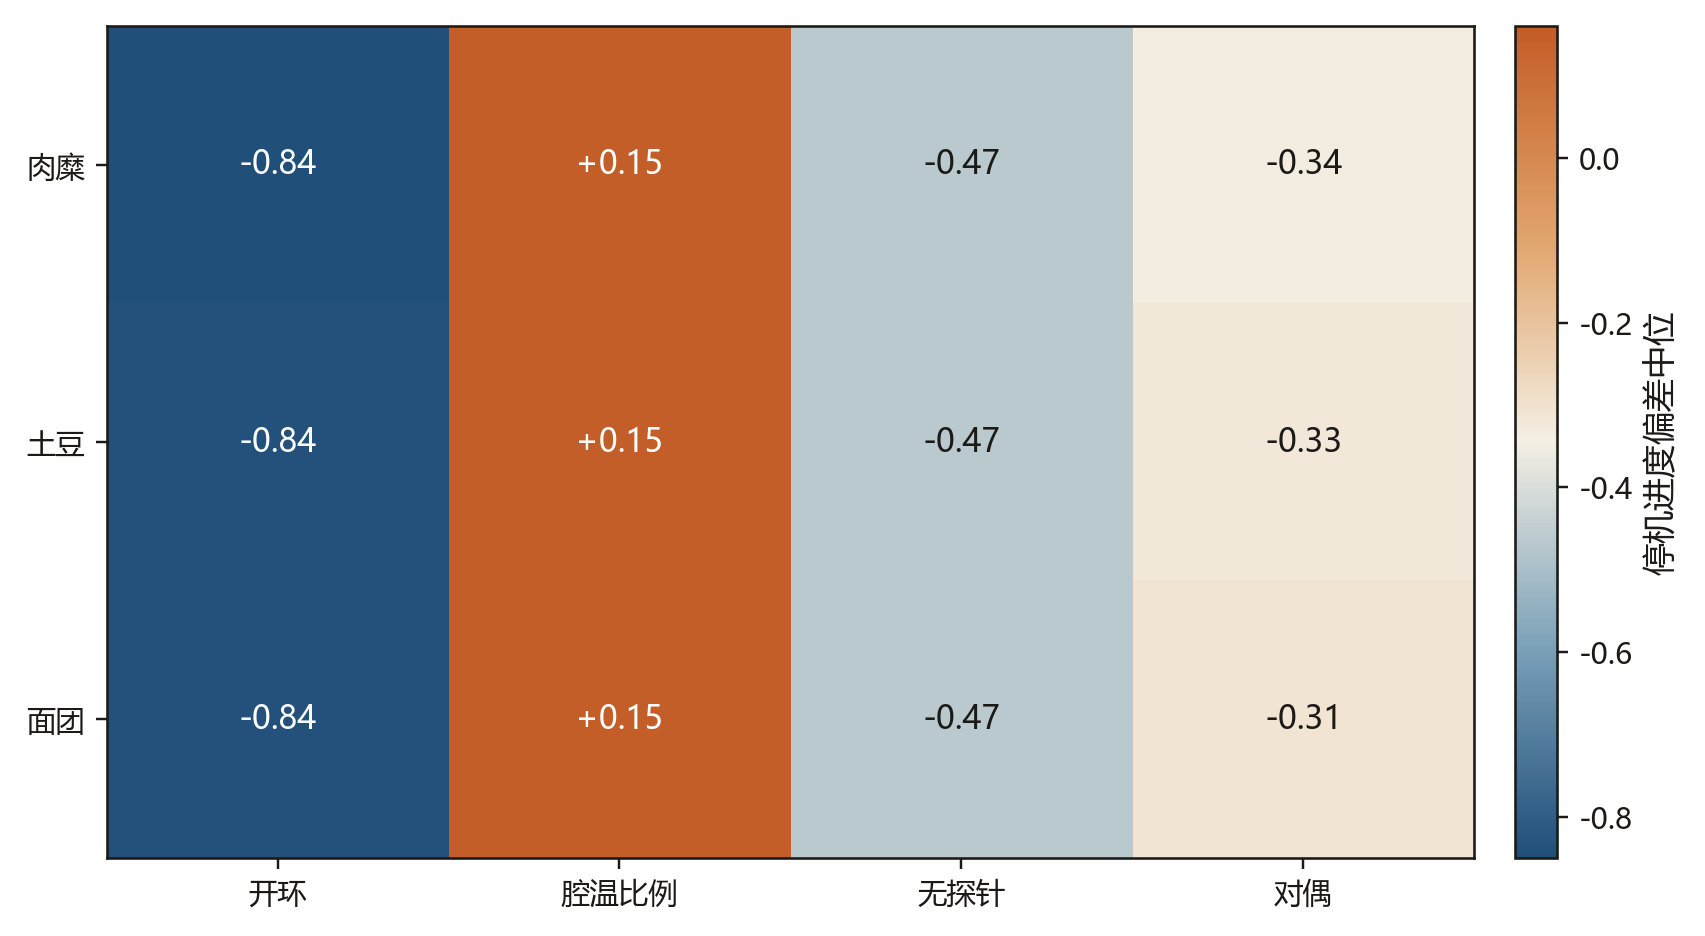
\includegraphics[width=0.86\textwidth]{D25_e_alpha.png}
\caption{D25。原型与策略的中位 \(e_{\alpha}\)。三个原型几乎相同，因为核里原型只改活度尺度。不能写成蛋白与淀粉的反应差异已经检验。}
\end{figure}

\begin{figure}[ht]
\centering
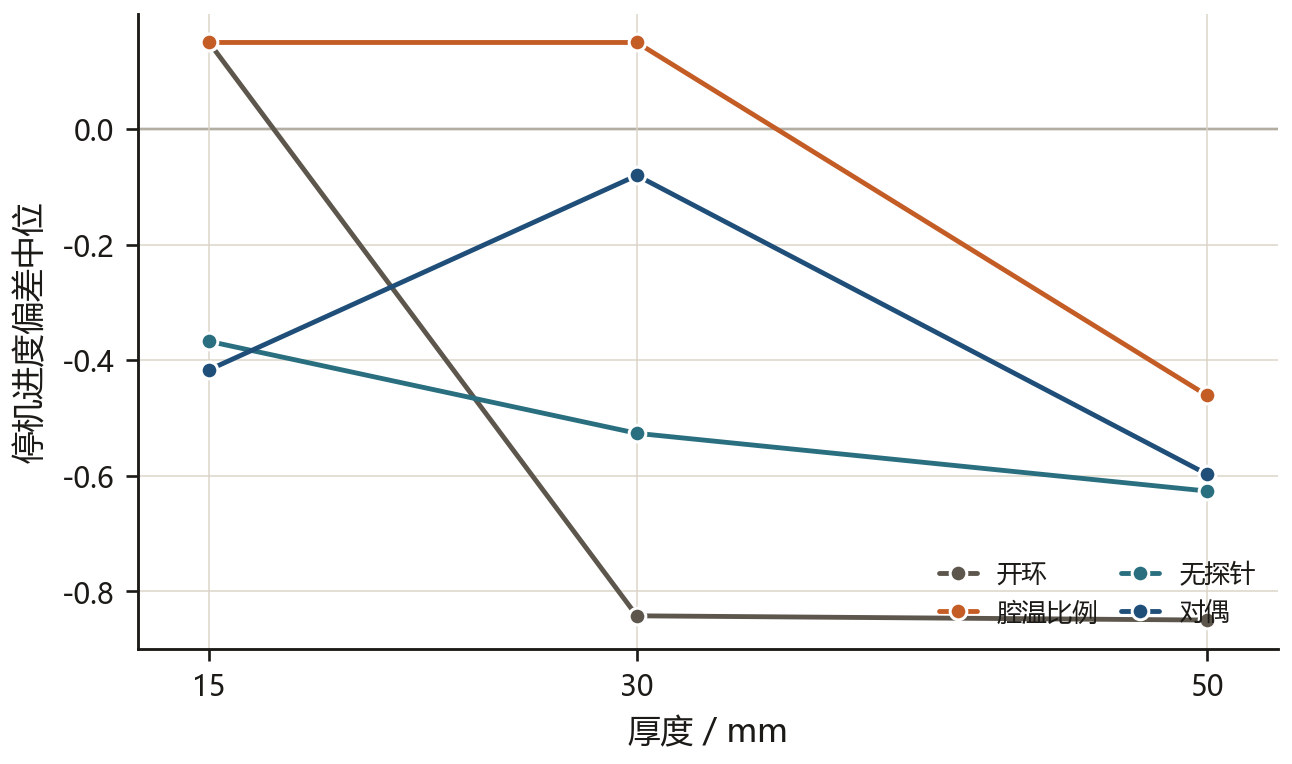
\includegraphics[width=0.86\textwidth]{D7_thickness.png}
\caption{D7。厚度与策略的进度误差。15 mm 的开环达到上沿；30 mm 的对偶中位数接近零而无探针仍明显为负；50 mm 两者都为负。不能外推到未运行的二维几何。}
\end{figure}

厚度把四个策略分开。箱线取自同一份摘要，离群点没有画出，所以须的端点是四分位以外的样本，不是全部样本的极值。

\begin{figure}[ht]
\centering
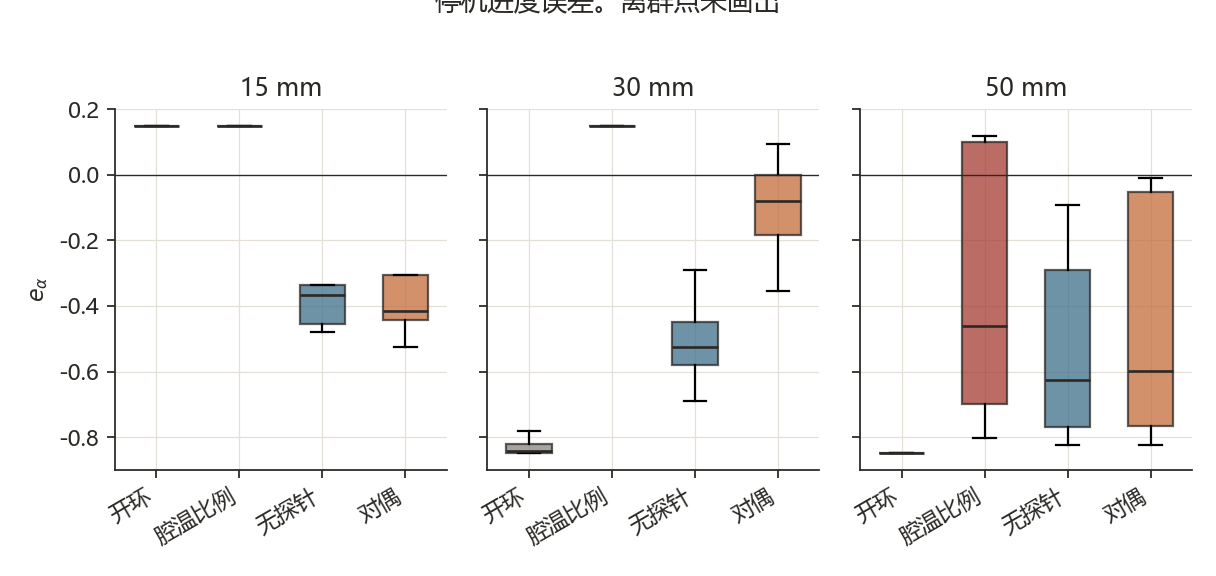
\includegraphics[width=\textwidth]{paper/P_box_thickness.png}
\caption{停机进度误差按厚度分开。15 mm 上对偶与无探针接近，开环和腔温比例贴在上沿。30 mm 上对偶的箱子跨过零线，无探针仍在零下。50 mm 上两者的中位数都在零下。腔温比例在 15 mm 与 30 mm 上贴住上沿，在 50 mm 上展开。}
\end{figure}

\begin{figure}[ht]
\centering
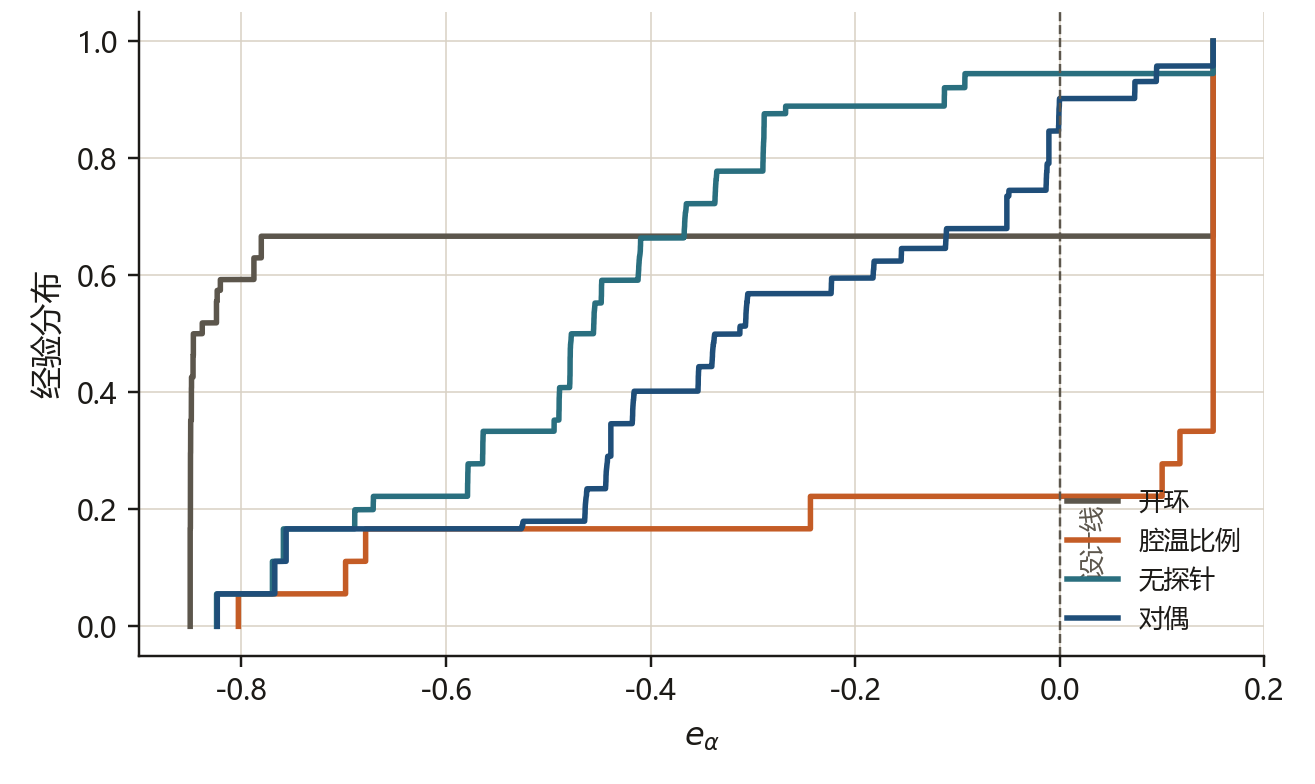
\includegraphics[width=0.92\textwidth]{paper/P_ecdf.png}
\caption{经验分布，每个策略 4860 条。零线是设计线。腔温比例在右端有一截竖起的质量，对应进度饱和。}
\end{figure}

\begin{figure}[ht]
\centering
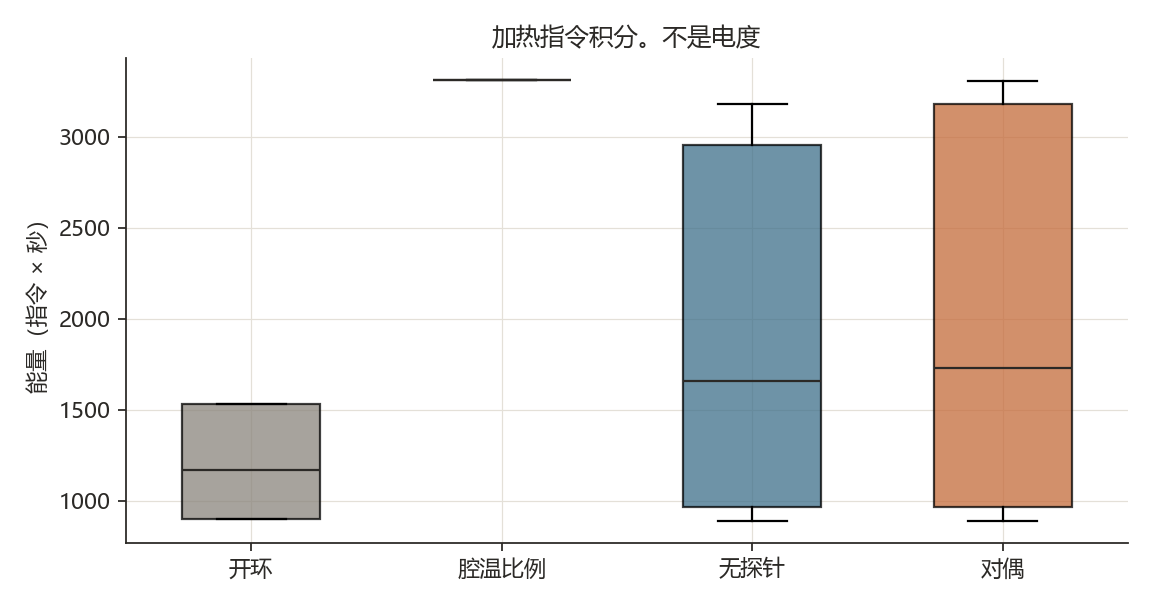
\includegraphics[width=0.86\textwidth]{paper/P_energy.png}
\caption{加热指令对记录间隔求和。开环最省，腔温比例最大。对偶略高于无探针。单位不是电度。}
\end{figure}

\begin{figure}[ht]
\centering
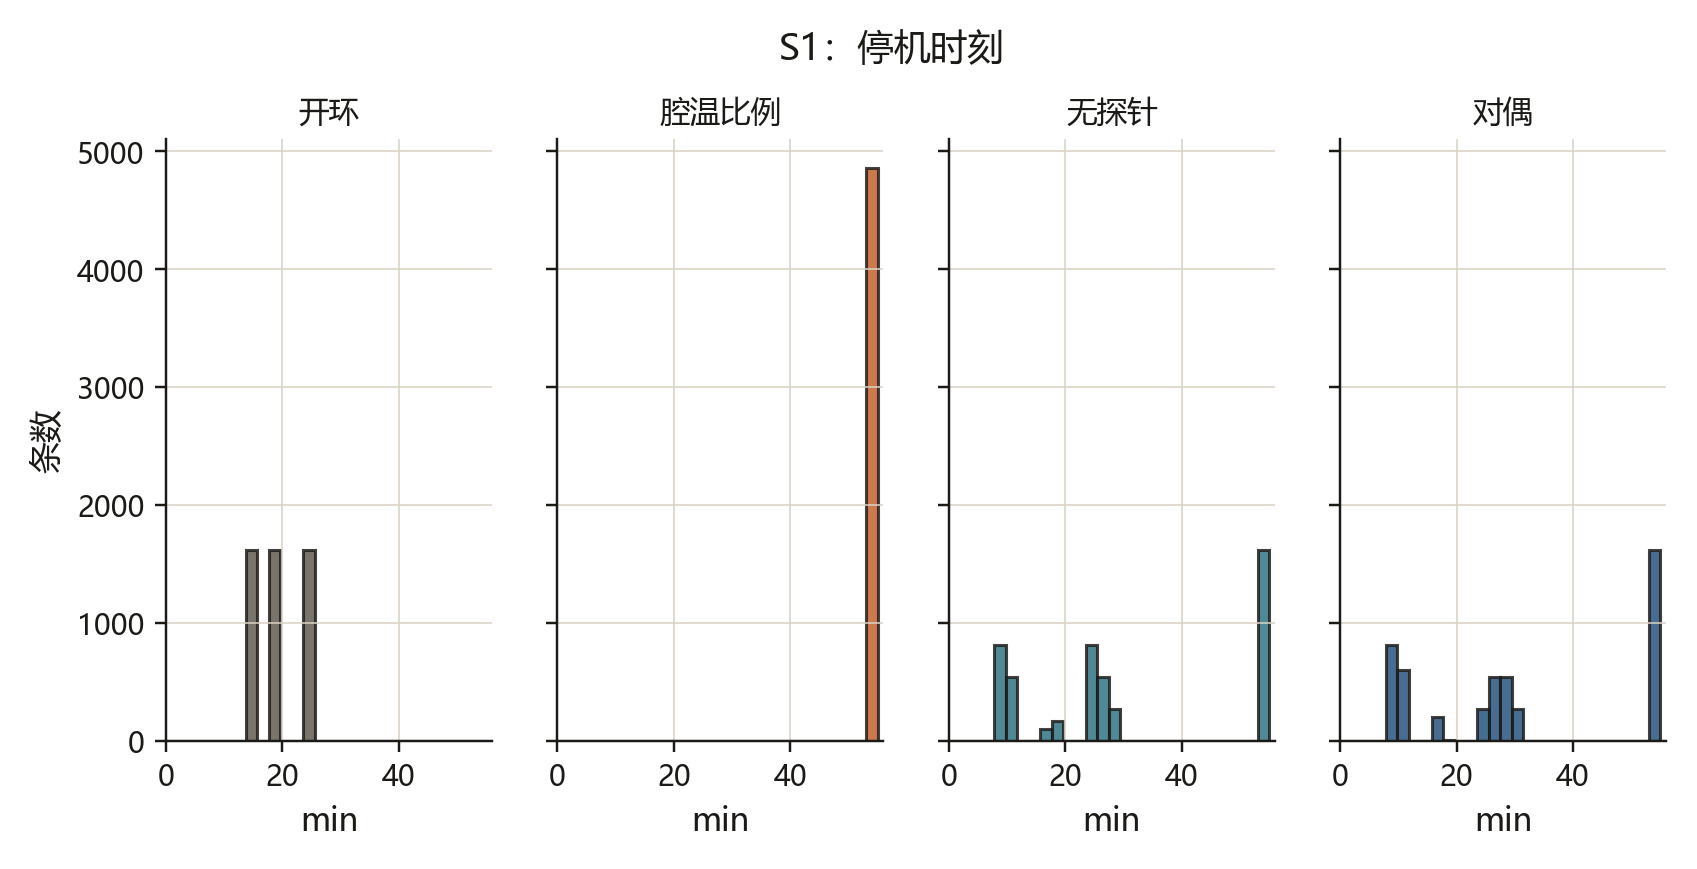
\includegraphics[width=\textwidth]{paper/P_stop.png}
\caption{停机时刻。开环集中在三档菜单时间。腔温比例全部停在时域终点。无探针与对偶的停机分布随厚度移动。}
\end{figure}

\begin{figure}[ht]
\centering
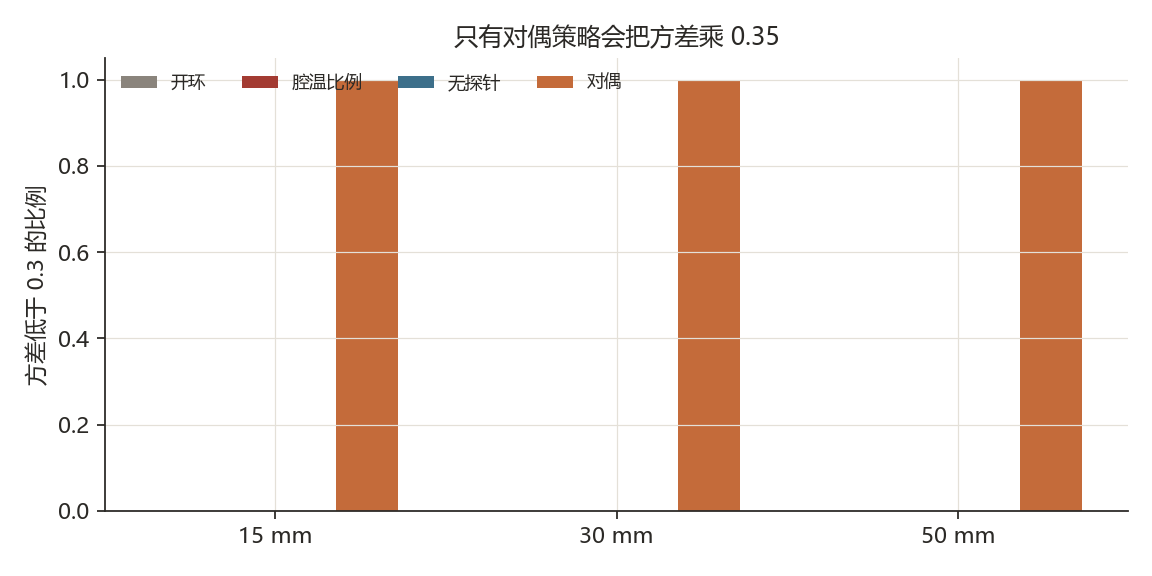
\includegraphics[width=0.86\textwidth]{paper/P_varr.png}
\caption{终点方差低于 0.3 的比例。只有对偶策略执行乘 0.35 的更新。另外三列是 0。}
\end{figure}

完整的分组中位数在下面的表里，来自同一份 \texttt{s1\_summary.json}。

\subsection{交叉表的读法}
表中每一行来自 \texttt{s1\_summary.json} 的分组中位数与分位。$e$ 是停机时 $\alpha_m-0.85$。$e{<}0$ 表示停在设计线之下。$e_{50}=0.150$ 且上尾贴住 $0.150$，是进度饱和到 $1$ 之后的上沿，不是测量精度。能量 $E$ 是加热指令对时间的求和，单位为指令$\times$秒，不是电度。全部记录 \texttt{augmented=false}，\texttt{source=simulation}。这些行是同一数值核的样本，不是独立烹饪实验。
\begin{longtable}{lrrrrrrr}
\caption{四个策略的总体}\\
\toprule
分组 & $n$ & $e_{10}$ & $e_{50}$ & $e_{90}$ & $P(e{<}0)$ & $E_{50}$ & $t_{50}$ \\
\midrule
\endfirsthead
\toprule
分组 & $n$ & $e_{10}$ & $e_{50}$ & $e_{90}$ & $P(e{<}0)$ & $E_{50}$ & $t_{50}$ \\
\midrule
\endhead
对偶 & 4860 & -0.767 & -0.313 & -0.000 & 0.902 & 1730 & 1641 \\
无探针 & 4860 & -0.770 & -0.467 & -0.113 & 0.944 & 1655 & 1540 \\
开环 & 4860 & -0.850 & -0.843 & 0.150 & 0.667 & 1170 & 1170 \\
腔温比例 & 4860 & -0.698 & 0.150 & 0.150 & 0.222 & 3310 & 3300 \\
\bottomrule
\end{longtable}

\begin{longtable}{lrrrrrrr}
\caption{食材与策略}\\
\toprule
分组 & $n$ & $e_{10}$ & $e_{50}$ & $e_{90}$ & $P(e{<}0)$ & $E_{50}$ & $t_{50}$ \\
\midrule
\endfirsthead
\toprule
分组 & $n$ & $e_{10}$ & $e_{50}$ & $e_{90}$ & $P(e{<}0)$ & $E_{50}$ & $t_{50}$ \\
\midrule
\endhead
面团, 对偶 & 1620 & -0.767 & -0.313 & 0.007 & 0.900 & 1730 & 1641 \\
面团, 无探针 & 1620 & -0.770 & -0.467 & -0.113 & 0.944 & 1655 & 1540 \\
面团, 开环 & 1620 & -0.850 & -0.836 & 0.150 & 0.667 & 1170 & 1170 \\
面团, 腔温比例 & 1620 & -0.698 & 0.150 & 0.150 & 0.222 & 3310 & 3300 \\
肉糜, 对偶 & 1620 & -0.767 & -0.338 & -0.000 & 0.904 & 1730 & 1641 \\
肉糜, 无探针 & 1620 & -0.770 & -0.467 & -0.113 & 0.944 & 1655 & 1540 \\
肉糜, 开环 & 1620 & -0.850 & -0.843 & 0.150 & 0.667 & 1170 & 1170 \\
肉糜, 腔温比例 & 1620 & -0.698 & 0.150 & 0.150 & 0.222 & 3310 & 3300 \\
土豆, 对偶 & 1620 & -0.767 & -0.325 & -0.000 & 0.902 & 1729 & 1641 \\
土豆, 无探针 & 1620 & -0.770 & -0.467 & -0.113 & 0.944 & 1655 & 1540 \\
土豆, 开环 & 1620 & -0.850 & -0.836 & 0.150 & 0.667 & 1170 & 1170 \\
土豆, 腔温比例 & 1620 & -0.698 & 0.150 & 0.150 & 0.222 & 3310 & 3300 \\
\bottomrule
\end{longtable}

\begin{longtable}{lrrrrrrr}
\caption{厚度与策略}\\
\toprule
分组 & $n$ & $e_{10}$ & $e_{50}$ & $e_{90}$ & $P(e{<}0)$ & $E_{50}$ & $t_{50}$ \\
\midrule
\endfirsthead
\toprule
分组 & $n$ & $e_{10}$ & $e_{50}$ & $e_{90}$ & $P(e{<}0)$ & $E_{50}$ & $t_{50}$ \\
\midrule
\endhead
15.0, 对偶 & 1620 & -0.464 & -0.417 & 0.150 & 0.872 & 932 & 591 \\
15.0, 无探针 & 1620 & -0.478 & -0.367 & 0.150 & 0.833 & 933 & 594 \\
15.0, 开环 & 1620 & 0.150 & 0.150 & 0.150 & 0.000 & 900 & 900 \\
15.0, 腔温比例 & 1620 & 0.150 & 0.150 & 0.150 & 0.000 & 3310 & 3300 \\
30.0, 对偶 & 1620 & -0.353 & -0.080 & 0.073 & 0.833 & 1730 & 1641 \\
30.0, 无探针 & 1620 & -0.671 & -0.527 & -0.290 & 1.000 & 1655 & 1540 \\
30.0, 开环 & 1620 & -0.849 & -0.843 & -0.780 & 1.000 & 1170 & 1170 \\
30.0, 腔温比例 & 1620 & 0.150 & 0.150 & 0.150 & 0.000 & 3310 & 3300 \\
50.0, 对偶 & 1620 & -0.823 & -0.598 & -0.011 & 1.000 & 3250 & 3300 \\
50.0, 无探针 & 1620 & -0.824 & -0.627 & -0.113 & 1.000 & 3055 & 3292 \\
50.0, 开环 & 1620 & -0.850 & -0.850 & -0.850 & 1.000 & 1530 & 1530 \\
50.0, 腔温比例 & 1620 & -0.803 & -0.461 & 0.117 & 0.667 & 3310 & 3300 \\
\bottomrule
\end{longtable}

\begin{longtable}{lrrrrrrr}
\caption{食材、厚度与策略}\\
\toprule
分组 & $n$ & $e_{10}$ & $e_{50}$ & $e_{90}$ & $P(e{<}0)$ & $E_{50}$ & $t_{50}$ \\
\midrule
\endfirsthead
\toprule
分组 & $n$ & $e_{10}$ & $e_{50}$ & $e_{90}$ & $P(e{<}0)$ & $E_{50}$ & $t_{50}$ \\
\midrule
\endhead
面团, 15.0, 对偶 & 540 & -0.464 & -0.416 & 0.150 & 0.867 & 932 & 592 \\
面团, 15.0, 无探针 & 540 & -0.478 & -0.367 & 0.150 & 0.833 & 933 & 594 \\
面团, 15.0, 开环 & 540 & 0.150 & 0.150 & 0.150 & 0.000 & 900 & 900 \\
面团, 15.0, 腔温比例 & 540 & 0.150 & 0.150 & 0.150 & 0.000 & 3310 & 3300 \\
面团, 30.0, 对偶 & 540 & -0.353 & -0.080 & 0.073 & 0.833 & 1730 & 1641 \\
面团, 30.0, 无探针 & 540 & -0.689 & -0.527 & -0.290 & 1.000 & 1655 & 1540 \\
面团, 30.0, 开环 & 540 & -0.849 & -0.836 & -0.780 & 1.000 & 1170 & 1170 \\
面团, 30.0, 腔温比例 & 540 & 0.150 & 0.150 & 0.150 & 0.000 & 3310 & 3300 \\
面团, 50.0, 对偶 & 540 & -0.823 & -0.598 & -0.011 & 1.000 & 3250 & 3300 \\
面团, 50.0, 无探针 & 540 & -0.824 & -0.627 & -0.113 & 1.000 & 3053 & 3291 \\
面团, 50.0, 开环 & 540 & -0.850 & -0.850 & -0.850 & 1.000 & 1530 & 1530 \\
面团, 50.0, 腔温比例 & 540 & -0.803 & -0.461 & 0.117 & 0.667 & 3310 & 3300 \\
肉糜, 15.0, 对偶 & 540 & -0.464 & -0.417 & 0.150 & 0.878 & 932 & 591 \\
肉糜, 15.0, 无探针 & 540 & -0.478 & -0.367 & 0.150 & 0.833 & 933 & 594 \\
肉糜, 15.0, 开环 & 540 & 0.150 & 0.150 & 0.150 & 0.000 & 900 & 900 \\
肉糜, 15.0, 腔温比例 & 540 & 0.150 & 0.150 & 0.150 & 0.000 & 3310 & 3300 \\
肉糜, 30.0, 对偶 & 540 & -0.353 & -0.080 & 0.073 & 0.833 & 1730 & 1641 \\
肉糜, 30.0, 无探针 & 540 & -0.671 & -0.527 & -0.290 & 1.000 & 1655 & 1540 \\
肉糜, 30.0, 开环 & 540 & -0.850 & -0.843 & -0.821 & 1.000 & 1170 & 1170 \\
肉糜, 30.0, 腔温比例 & 540 & 0.150 & 0.150 & 0.150 & 0.000 & 3310 & 3300 \\
肉糜, 50.0, 对偶 & 540 & -0.823 & -0.598 & -0.011 & 1.000 & 3250 & 3300 \\
肉糜, 50.0, 无探针 & 540 & -0.824 & -0.627 & -0.113 & 1.000 & 3055 & 3292 \\
肉糜, 50.0, 开环 & 540 & -0.850 & -0.850 & -0.850 & 1.000 & 1530 & 1530 \\
肉糜, 50.0, 腔温比例 & 540 & -0.803 & -0.461 & 0.117 & 0.667 & 3310 & 3300 \\
土豆, 15.0, 对偶 & 540 & -0.464 & -0.417 & 0.150 & 0.872 & 932 & 591 \\
土豆, 15.0, 无探针 & 540 & -0.478 & -0.367 & 0.150 & 0.833 & 933 & 594 \\
土豆, 15.0, 开环 & 540 & 0.150 & 0.150 & 0.150 & 0.000 & 900 & 900 \\
土豆, 15.0, 腔温比例 & 540 & 0.150 & 0.150 & 0.150 & 0.000 & 3310 & 3300 \\
土豆, 30.0, 对偶 & 540 & -0.353 & -0.080 & 0.073 & 0.833 & 1729 & 1641 \\
土豆, 30.0, 无探针 & 540 & -0.671 & -0.527 & -0.290 & 1.000 & 1655 & 1540 \\
土豆, 30.0, 开环 & 540 & -0.849 & -0.836 & -0.780 & 1.000 & 1170 & 1170 \\
土豆, 30.0, 腔温比例 & 540 & 0.150 & 0.150 & 0.150 & 0.000 & 3310 & 3300 \\
土豆, 50.0, 对偶 & 540 & -0.823 & -0.598 & -0.011 & 1.000 & 3249 & 3300 \\
土豆, 50.0, 无探针 & 540 & -0.824 & -0.627 & -0.113 & 1.000 & 3055 & 3292 \\
土豆, 50.0, 开环 & 540 & -0.850 & -0.850 & -0.850 & 1.000 & 1530 & 1530 \\
土豆, 50.0, 腔温比例 & 540 & -0.803 & -0.461 & 0.117 & 0.667 & 3310 & 3300 \\
\bottomrule
\end{longtable}

\begin{longtable}{lrrrrrrr}
\caption{非均质档、厚度与策略}\\
\toprule
分组 & $n$ & $e_{10}$ & $e_{50}$ & $e_{90}$ & $P(e{<}0)$ & $E_{50}$ & $t_{50}$ \\
\midrule
\endfirsthead
\toprule
分组 & $n$ & $e_{10}$ & $e_{50}$ & $e_{90}$ & $P(e{<}0)$ & $E_{50}$ & $t_{50}$ \\
\midrule
\endhead
0, 15.0, 对偶 & 540 & -0.444 & -0.391 & -0.338 & 1.000 & 924 & 578 \\
0, 15.0, 无探针 & 540 & -0.479 & -0.422 & -0.365 & 1.000 & 925 & 580 \\
0, 15.0, 开环 & 540 & 0.150 & 0.150 & 0.150 & 0.000 & 900 & 900 \\
0, 15.0, 腔温比例 & 540 & 0.150 & 0.150 & 0.150 & 0.000 & 3310 & 3300 \\
0, 30.0, 对偶 & 540 & -0.155 & -0.080 & -0.013 & 1.000 & 1714 & 1617 \\
0, 30.0, 无探针 & 540 & -0.579 & -0.513 & -0.410 & 1.000 & 1640 & 1516 \\
0, 30.0, 开环 & 540 & -0.849 & -0.835 & -0.788 & 1.000 & 1170 & 1170 \\
0, 30.0, 腔温比例 & 540 & 0.150 & 0.150 & 0.150 & 0.000 & 3310 & 3300 \\
0, 50.0, 对偶 & 540 & -0.767 & -0.409 & -0.052 & 1.000 & 3229 & 3300 \\
0, 50.0, 无探针 & 540 & -0.770 & -0.529 & -0.268 & 1.000 & 3024 & 3249 \\
0, 50.0, 开环 & 540 & -0.850 & -0.850 & -0.850 & 1.000 & 1530 & 1530 \\
0, 50.0, 腔温比例 & 540 & -0.698 & -0.299 & 0.100 & 0.500 & 3310 & 3300 \\
1, 15.0, 对偶 & 540 & -0.418 & -0.362 & -0.305 & 1.000 & 931 & 583 \\
1, 15.0, 无探针 & 540 & -0.456 & -0.352 & -0.336 & 1.000 & 932 & 584 \\
1, 15.0, 开环 & 540 & 0.150 & 0.150 & 0.150 & 0.000 & 900 & 900 \\
1, 15.0, 腔温比例 & 540 & 0.150 & 0.150 & 0.150 & 0.000 & 3310 & 3300 \\
1, 30.0, 对偶 & 540 & -0.001 & 0.036 & 0.095 & 0.500 & 1741 & 1643 \\
1, 30.0, 无探针 & 540 & -0.489 & -0.390 & -0.289 & 1.000 & 1664 & 1539 \\
1, 30.0, 开环 & 540 & -0.849 & -0.834 & -0.780 & 1.000 & 1170 & 1170 \\
1, 30.0, 腔温比例 & 540 & 0.150 & 0.150 & 0.150 & 0.000 & 3310 & 3300 \\
1, 50.0, 对偶 & 540 & -0.756 & -0.383 & -0.011 & 1.000 & 3255 & 3300 \\
1, 50.0, 无探针 & 540 & -0.759 & -0.436 & -0.093 & 1.000 & 3071 & 3281 \\
1, 50.0, 开环 & 540 & -0.850 & -0.850 & -0.850 & 1.000 & 1530 & 1530 \\
1, 50.0, 腔温比例 & 540 & -0.678 & -0.280 & 0.117 & 0.500 & 3310 & 3300 \\
2, 15.0, 对偶 & 540 & -0.525 & -0.463 & 0.150 & 0.617 & 941 & 607 \\
2, 15.0, 无探针 & 540 & -0.412 & -0.130 & 0.150 & 0.500 & 988 & 799 \\
2, 15.0, 开环 & 540 & 0.150 & 0.150 & 0.150 & 0.000 & 900 & 900 \\
2, 15.0, 腔温比例 & 540 & 0.150 & 0.150 & 0.150 & 0.000 & 3310 & 3300 \\
2, 30.0, 对偶 & 540 & -0.353 & -0.268 & -0.182 & 1.000 & 1749 & 1670 \\
2, 30.0, 无探针 & 540 & -0.689 & -0.618 & -0.564 & 1.000 & 1674 & 1568 \\
2, 30.0, 开环 & 540 & -0.850 & -0.844 & -0.824 & 1.000 & 1170 & 1170 \\
2, 30.0, 腔温比例 & 540 & 0.150 & 0.150 & 0.150 & 0.000 & 3310 & 3300 \\
2, 50.0, 对偶 & 540 & -0.823 & -0.631 & -0.439 & 1.000 & 3245 & 3300 \\
2, 50.0, 无探针 & 540 & -0.824 & -0.659 & -0.479 & 1.000 & 3066 & 3292 \\
2, 50.0, 开环 & 540 & -0.850 & -0.850 & -0.850 & 1.000 & 1530 & 1530 \\
2, 50.0, 腔温比例 & 540 & -0.803 & -0.523 & -0.244 & 1.000 & 3310 & 3300 \\
\bottomrule
\end{longtable}

\begin{longtable}{lrrrrrrr}
\caption{初始含水与策略}\\
\toprule
分组 & $n$ & $e_{10}$ & $e_{50}$ & $e_{90}$ & $P(e{<}0)$ & $E_{50}$ & $t_{50}$ \\
\midrule
\endfirsthead
\toprule
分组 & $n$ & $e_{10}$ & $e_{50}$ & $e_{90}$ & $P(e{<}0)$ & $E_{50}$ & $t_{50}$ \\
\midrule
\endhead
0.64, 对偶 & 1620 & -0.767 & -0.313 & -0.000 & 0.902 & 1730 & 1641 \\
0.64, 无探针 & 1620 & -0.770 & -0.467 & -0.113 & 0.944 & 1655 & 1540 \\
0.64, 开环 & 1620 & -0.850 & -0.843 & 0.150 & 0.667 & 1170 & 1170 \\
0.64, 腔温比例 & 1620 & -0.698 & 0.150 & 0.150 & 0.222 & 3310 & 3300 \\
0.72, 对偶 & 1620 & -0.767 & -0.313 & -0.000 & 0.902 & 1730 & 1641 \\
0.72, 无探针 & 1620 & -0.770 & -0.467 & -0.113 & 0.944 & 1655 & 1540 \\
0.72, 开环 & 1620 & -0.850 & -0.843 & 0.150 & 0.667 & 1170 & 1170 \\
0.72, 腔温比例 & 1620 & -0.698 & 0.150 & 0.150 & 0.222 & 3310 & 3300 \\
0.8, 对偶 & 1620 & -0.767 & -0.313 & -0.000 & 0.902 & 1730 & 1641 \\
0.8, 无探针 & 1620 & -0.770 & -0.467 & -0.113 & 0.944 & 1655 & 1540 \\
0.8, 开环 & 1620 & -0.850 & -0.843 & 0.150 & 0.667 & 1170 & 1170 \\
0.8, 腔温比例 & 1620 & -0.698 & 0.150 & 0.150 & 0.222 & 3310 & 3300 \\
\bottomrule
\end{longtable}

\begin{longtable}{lrrrrrrr}
\caption{初始温度与策略}\\
\toprule
分组 & $n$ & $e_{10}$ & $e_{50}$ & $e_{90}$ & $P(e{<}0)$ & $E_{50}$ & $t_{50}$ \\
\midrule
\endfirsthead
\toprule
分组 & $n$ & $e_{10}$ & $e_{50}$ & $e_{90}$ & $P(e{<}0)$ & $E_{50}$ & $t_{50}$ \\
\midrule
\endhead
5.0, 对偶 & 2430 & -0.823 & -0.417 & -0.000 & 0.915 & 1822 & 1740 \\
5.0, 无探针 & 2430 & -0.824 & -0.579 & 0.150 & 0.889 & 1738 & 1628 \\
5.0, 开环 & 2430 & -0.850 & -0.849 & 0.150 & 0.667 & 1170 & 1170 \\
5.0, 腔温比例 & 2430 & -0.803 & 0.150 & 0.150 & 0.333 & 3310 & 3300 \\
20.0, 对偶 & 2430 & -0.463 & -0.182 & 0.073 & 0.889 & 1658 & 1544 \\
20.0, 无探针 & 2430 & -0.564 & -0.366 & -0.113 & 1.000 & 1587 & 1448 \\
20.0, 开环 & 2430 & -0.850 & -0.821 & 0.150 & 0.667 & 1170 & 1170 \\
20.0, 腔温比例 & 2430 & -0.244 & 0.150 & 0.150 & 0.111 & 3310 & 3300 \\
\bottomrule
\end{longtable}


读表时只增加图里没有写完的比较。初始含水三档在表的精度上逐格相同：对偶都是 \(e_{10}=-0.767\)、\(e_{50}=-0.313\)、提前比例 0.902、能量 1730、停机 1641。含水没有进入这一批停机误差，与活度在这三档上饱和一致。初温不改变四个策略中位数的次序，但改变幅度。对偶在 \(5^\circ\mathrm{C}\) 的中位数是 \(-0.417\)、能量 1822、停机 1740；在 \(20^\circ\mathrm{C}\) 是 \(-0.182\)、能量 1658、停机 1544。腔温比例的提前比例从 0.333 降到 0.111。厚度仍然把排序拉开得更明显。

非均质档 2 把一个控制体的导热降低，厚件的提前没有因此消失。30 mm、对偶、均匀时 \(e_{50}=-0.080\)、提前比例 1；同一厚度、对偶、初始温度倾斜 \(\pm 4^\circ\mathrm{C}\) 时 \(e_{50}=+0.036\)、提前比例降到 0.5；同一厚度、对偶、导热缺损时 \(e_{50}=-0.268\)、提前比例仍是 1。倾斜改变的是初值，不是边界驱动的冷点迁移。表中的能量单位是加热指令乘以记录间隔 10 s，不是电度。停止时刻的中位数与菜单时间在开环上重合：15 mm 为 900 s，30 mm 为 1170 s，50 mm 为 1530 s，说明开环确实停在菜单终点。腔温比例的能量中位数 3310 是 331 个记录点各乘 10 s，请求被裁在 1 上，与食材和厚度无关。

\subsection{同一格里的三十个种子}

648 个格子各有 30 个种子。开环的 162 格和腔温比例的 162 格，格内 \(e_{\alpha}\) 的极差都是 0：三十个种子写出同一个停机误差。无探针 162 格的极差中位数是 0.0018，九十分位是 0.0385，最大是 0.0883，极差为 0 的格子占 0.222。对偶 162 格的极差中位数是 0.0021，九十分位是 0.0442，极差为 0 的格子占 0.333。

极差大于 0.05 的格子只有 18 个，全部在 15 mm、初温 \(5^\circ\mathrm{C}\)。对偶的 9 个都是导热缺损。无探针的 9 个都是初始温度倾斜，极差 0.088，中位数 \(-0.455\)，区间 \([-0.456,-0.367]\)。三种含水的计数完全相同，含水仍然不进入这一列。

对偶、导热缺损这一档里，食材只改变两簇的人数。肉糜是 22 个种子停在 \(+0.150\)、8 个停在约 \(-0.525\)。土豆是 23 与 7。面团是 24 与 6。下面只画肉糜、含水 0.72 的 30 个种子。负的一簇停在 650 s 或 652 s，能量从 975.5 到 978.1。正的一簇停在 1010 s 到 1066 s，能量从 1060.3 到 1072.3。中位数 \(+0.150\) 落在人数多的那一簇上，8 条停在设计线之下约 0.525 的轨迹不改变这个中位数。

\begin{figure}[ht]
\centering
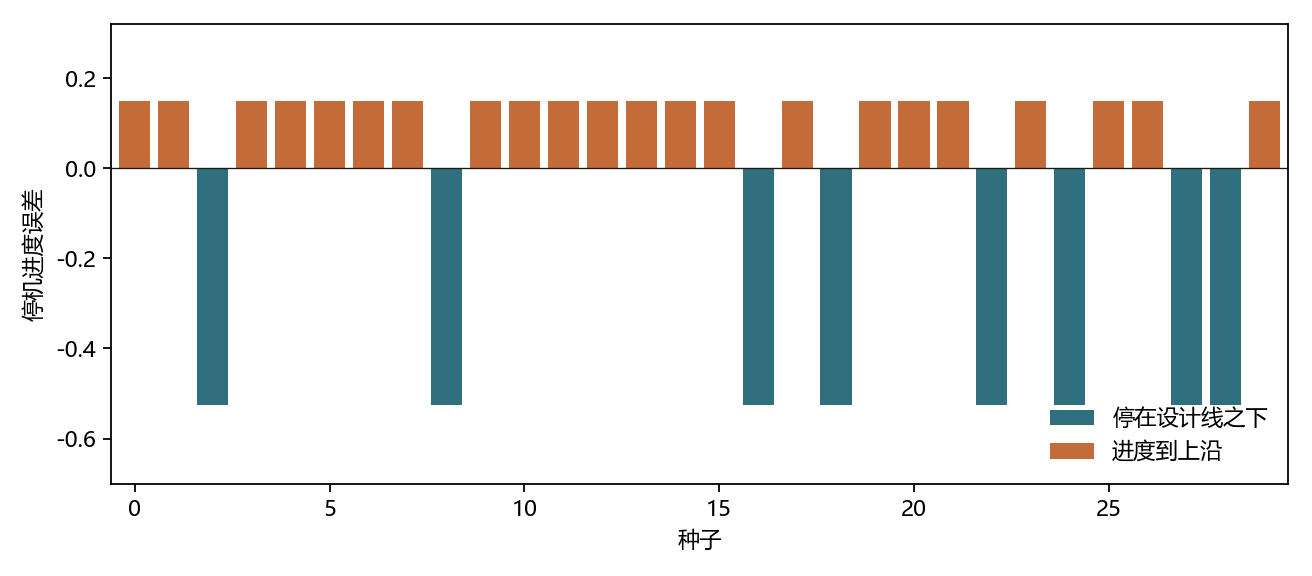
\includegraphics[width=\textwidth]{paper/P_seed_cell.png}
\caption{15 mm、初温 \(5^\circ\mathrm{C}\)、导热缺损、对偶、肉糜、含水 0.72 的 30 个种子。橙色停在进度上沿，青绿色停在设计线之下。这是种子把停机误差分成两簇的一档。其余格子的极差接近 0，分位数几乎是同一个数重复三十次。}
\end{figure}

\paragraph{本节不能推出的结论}
这一格分成两簇，不能改写中位数的定义，也不能写成噪声模型已经标定。它只说明：这一格的中位数对人数敏感。另外 630 个格子的格内极差都不超过 0.05。终点方差不在这些种子之间变化：对偶全部是 0.224，另外三个策略全部是 0.64。褐变终点全部是 0。

\section{网格减半}

S0 的 18 条配对都是对偶、30 mm、初温 \(5^\circ\mathrm{C}\)、含水 0.72、均匀。16 个控制体的 \(e_{\alpha}\) 中位数是 \(-0.112\)，停止时刻落在 1714 s 到 1718 s。8 个控制体的中位数是 \(+0.116\)，停止时刻落在 1746 s 到 1750 s。差值 \(e_8-e_{16}\) 的中位数是 \(+0.227\)，最小 \(0.227\)，最大 \(0.270\)。三种食品没有把这个差拉开。

\begin{figure}[ht]
\centering
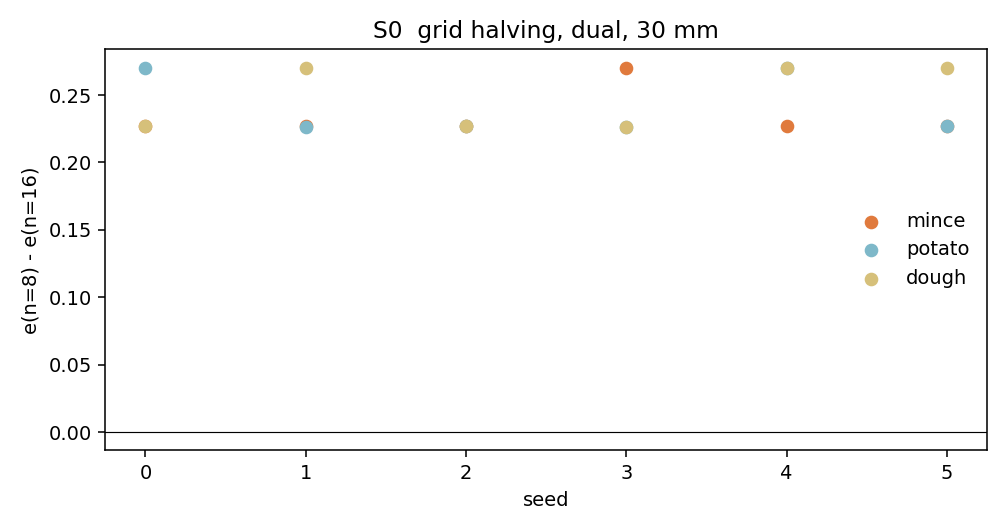
\includegraphics[width=0.86\textwidth]{S0_grid.png}
\caption{S0。网格从 16 个控制体减到 8 个之后，同一 30 mm 对偶设定的停机误差上升约 0.23。这是格式差，不是策略差。}
\end{figure}

差大于零，说明这一档的停机误差随网格改变。它没有低于一个事先写死的决策阈值，因为规格只说“低于阈值”，没有给出这个核上的数值。因此 S0 的结论是：16 个控制体的中位数不能当成网格无关。S1 的句子仍然以 16 个控制体为归属。

\paragraph{本节不能推出的结论}
网格减半改变 \(e_{\alpha}\)，不能写成 32 个控制体已经收敛，也不能写成二维截面会给出同一个差。

\section{边界扫描}

S2 的基准是肉糜、30 mm、初温 \(5^\circ\mathrm{C}\)、含水 0.72、对偶、40 个种子。中位 \(e_{\alpha}=-0.112\)，终点方差 0.224，提前比例为 1。同一基准上去掉探针，改走无探针，中位数降到 \(-0.579\)，终点方差留在 0.64。探针窗在这 40 个种子上都把方差乘了 0.35，但停机误差仍在设计线之下。

表面读数保持初值的时间从 0 增到 60 s 时，中位数从 \(-0.112\) 变到 \(-0.111\)、\(-0.110\)、\(-0.067\)。60 s 的保持让误差少负一点，没有跨过零。质量通道打开或关掉，中位数都是 \(-0.112\)，因为对偶不读这条通道。脂肪层把中位数从 \(-0.112\) 降到 \(-0.353\)。300 s 开门一次，中位数从 \(-0.112\) 降到 \(-0.151\)。终点方差在这些档上仍是 0.224：遮挡、脂肪和开门都没有挡住窗内那一次更新。

\begin{figure}[ht]
\centering
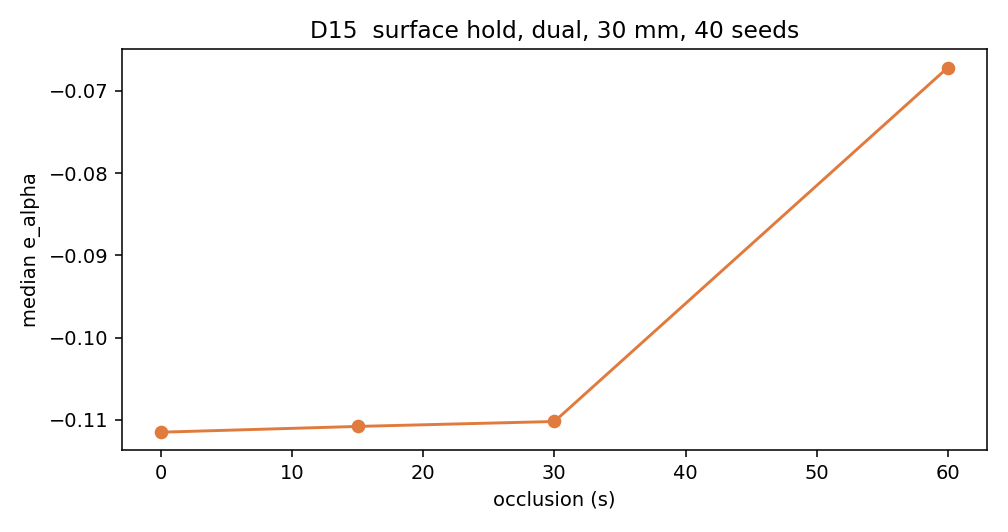
\includegraphics[width=0.86\textwidth]{D15_occlusion.png}
\caption{D15。表面读数在开局后保持初值的秒数，对照 40 个种子的中位停机误差。60 s 仍在零下。这不是热像遮挡的测量，核没有热像通道。}
\end{figure}

\begin{figure}[ht]
\centering
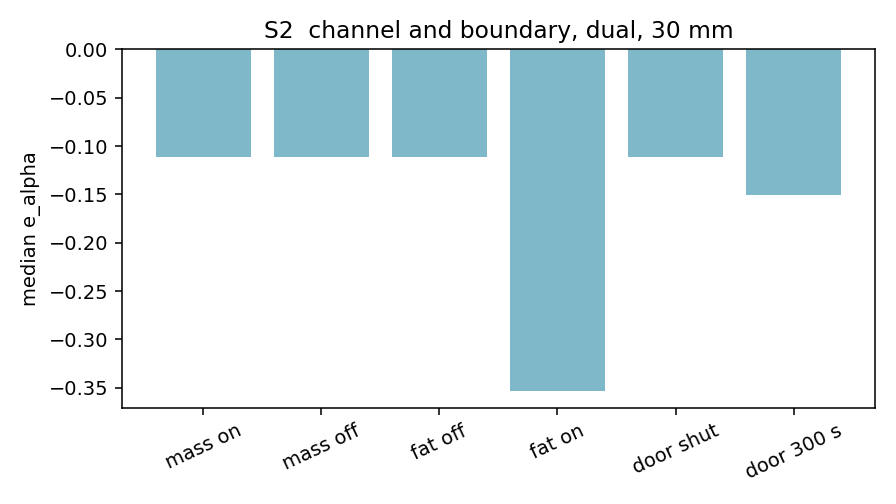
\includegraphics[width=\textwidth]{S2_factors.png}
\caption{S2。同一 30 mm 对偶基准上，质量通道不改变中位数，脂肪层和一次开门把它拉低。柱是 40 个种子的中位数。}
\end{figure}

\paragraph{本节不能推出的结论}
这一条 30 mm 设定上的差，不能外推到 15 mm 和 50 mm，也不能写成安全屏障已经被注入。噪声倍数没有单独扫描。

\section{能量、方差与褐变的伴随量}
下列数字由 \texttt{s1\_summary.json} 的 19440 行重新分组。能量仍是加热指令乘记录间隔。方差低于 0.3 表示走过一次乘 0.35 的更新；未更新的先验方差是 0.64。褐变是终点 $\alpha_b$，不是停机时刻。
\begin{longtable}{lrrrrrr}
\caption{按厚度与策略的能量分位与终点方差}\\
\toprule
分组 & $n$ & $E_{10}$ & $E_{50}$ & $E_{90}$ & 方差$<0.3$ & $\alpha_{b,50}$ \\
\midrule\endfirsthead
\toprule 分组 & $n$ & $E_{10}$ & $E_{50}$ & $E_{90}$ & 方差$<0.3$ & $\alpha_{b,50}$ \\\midrule\endhead
15\,mm, 开环 & 1620 & 900 & 900 & 900 & 0.000 & 0.0000 \\
15\,mm, 腔温比例 & 1620 & 3310 & 3310 & 3310 & 0.000 & 0.0000 \\
15\,mm, 无探针 & 1620 & 892 & 933 & 1076 & 0.000 & 0.0000 \\
15\,mm, 对偶 & 1620 & 890 & 932 & 1064 & 1.000 & 0.0000 \\
30\,mm, 开环 & 1620 & 1170 & 1170 & 1170 & 0.000 & 0.0000 \\
30\,mm, 腔温比例 & 1620 & 3310 & 3310 & 3310 & 0.000 & 0.0000 \\
30\,mm, 无探针 & 1620 & 1563 & 1655 & 1753 & 0.000 & 0.0000 \\
30\,mm, 对偶 & 1620 & 1629 & 1730 & 1836 & 1.000 & 0.0000 \\
50\,mm, 开环 & 1620 & 1530 & 1530 & 1530 & 0.000 & 0.0000 \\
50\,mm, 腔温比例 & 1620 & 3310 & 3310 & 3310 & 0.000 & 0.0000 \\
50\,mm, 无探针 & 1620 & 2901 & 3055 & 3178 & 0.000 & 0.0000 \\
50\,mm, 对偶 & 1620 & 3157 & 3250 & 3307 & 1.000 & 0.0000 \\
\bottomrule\end{longtable}
对偶在三档厚度上的方差下降比例都是 1。开环、腔温比例和无探针的比例是 0，因为它们的代码路径不写 $\hat r$。

终点褐变在这 19440 行里不是“中位数碰巧为零”。$\alpha_b$ 的最小值、十分位、中位数、九十分位和最大值都是 0，大于零的比例是 0。褐变增量要求表面含水低于 0.55，同时表面温度高于 $110^\circ\mathrm{C}$。S1 的初始含水是 0.64、0.72 和 0.80。表面失水项再乘上 $2\times 10^{-9}\,\mathrm{m}^2/\mathrm{s}$ 量级的扩散系数之后，下降率约为 $10^{-11}\,\mathrm{s}^{-1}$，3300 s 的下降量级是 $10^{-8}$。含水到不了 0.55，褐变增量在每一步都是 0，不是四位小数把一个小正数抹掉。结壳门限是 0.45，同样到不了，所以路径 C 里结壳增大热阻的那一支在这次战役里没有被积分。三个原型的活度在这三档含水上都贴着 0.99，表里的食材列因此也不能比较蛋白与淀粉的表面反应。

能量列里有一条与电功率无关的恒等式。战役记录间隔是 $2\,\mathrm{s}\times 5=10\,\mathrm{s}$，55 min 共 1650 步，记录点是 331 个。腔温比例把请求裁到 1，加热器平衡在 $196.5^\circ\mathrm{C}$，削减不动作，每个记录点的指令都是 1，能量就是 $331\times 10=3310$。开环在菜单终点把指令写成 0，900 s、1170 s、1530 s 都落在 10 s 网格上，能量中位数就等于菜单秒数。末步若不是记录步，代码仍把它记入，并仍乘满 10 s；3310 比 3300 多出的那一格是这个记账。


\paragraph{本节不能推出的结论}
表中任何一格都是数值样本。它不能出现在以“实验验证”为谓语的句子里。终点褐变中位数为 0，不能写成表面品质已经比较过。

\section{软件结构}

规格中的目录把真值步进、传感器、估计、探针、孪生、预测控制、算子和评价分开，评价与控制不共享内存中的真值对象。本次实现没有这些目录。积分、策略和评分在同一次循环里。评价能做的隔离只有：摘要文件在循环之后读取，图从摘要和一条演示轨迹生成。浏览器副本不读这份摘要。

噪声用正弦散列，不用随机数发生器，所以同一版本的代码重复运行得到同一日志。策略编号进入散列的相位，四个策略的噪声实现不相同。

\paragraph{本节不能推出的结论}
代码可复现，不能推出 16 个控制体已经网格无关。S0 的差约 0.23，写在网格减半一节。

\section{几何保真度的三档}

\begin{table}[ht]
\centering
\caption{几何档与本次归属}
\begin{tabularx}{\textwidth}{llX}
\toprule
档 & 规格 & 本次 \\
\midrule
T1 & 一维全因子，策略排序的主表 & 十六条控制体已运行，作为本章全部数字的归属 \\
T2 & 二维截面，脂肪夹层与各向异性 & 未运行。不能用档 2 的一个低导热控制体代替 \\
T3 & 风速与蒸汽的外部流动，只提供边界库 & 未运行。\(h\) 是线性式 \\
\bottomrule
\end{tabularx}
\end{table}

在线集合 32 与离线 128 没有运行。神经算子没有用 T1 训练，也没有在 T2 上做干预测试。一维结果不外推为整机三维热场。三维全耦合不在本章的结论内。

\paragraph{本章不能推出的结论}
主结论只限于：在这个一维核上，按厚度分开看，开环该薄的过了、该厚的没到；腔温比例靠持续加热把进度推到上沿，厚件仍有三分之二提前；无探针经常在真值进度未到设计线时停止；对偶在 30 mm 上把中位误差从约 \(-0.53\) 拉到约 \(-0.08\)，在 15 mm 上没有优势，在 50 mm 上两者都提前。S0 说明把控制体减半会把 30 mm 对偶的中位误差抬高约 0.23。S2 说明在同一条 30 mm 设定上，去掉探针、加上脂肪层或开一次门，都会把中位数拉得更低，而质量通道对对偶没有作用。这些句子的主语都是本核。它们不是多孔介质真值、不是集合滤波、也不是预测控制求解器的结果。
